\cleardoublepage
\singlespacing
\chapter{EVALUATION \& RESULTS}
\label{c:evaluation}
\doublespacing\nointerlineskip

%This chapter presents evaluation. The models and algorithms are
%tested extensively on benchmarks, which is described in
%section~\ref{s:benchmarks}, and the results are discussed in
%section~\ref{s:results}

In order to evaluate the performance of our fault tolerance system, we have
introduced some metrics to test how well it perform, and whether after node
failures requirements could still be met under small network.

\begin{enumerate}
\item Whether the next node in strip take over after failure
\item Memory overhead for Strips
\item Message overhead for failure recovery, including reconfiguration
\item Time to recover from failure
\end{enumerate}

Whenever a node failed, the the next node in the strips it is carrying would
take over for the respective services each represents.
Time to recover measures the time it takes to recover from the time of failure
detection.

We measured system performance live by collecting data from sensor nodes while
running. Sensor nodes are programmed to send out their tracking data to
a central data sink at appropriate times such as after node initialization or
when the failure is resolved.

The application, fault tolerance policy, network topology are described in the
following sections.


\section{Application}

Application shown in Figure~\ref{fig:fbp-application} will be deployed.  There
will be four components: 

\begin{enumerate}
\item Numeric Controller is a user input device which outputs
a number from 0 to 255. Light Sensor is a photodetector sensor which detects the
level of light intensity. 
\item Threshold is a conditional function which takes two
inputs, Threshold and Value, and, depending on the Operator attribute, return
true if the Operator is set to GT (Greater Than) and the Value is higher than
the Threshold. 
\item Light Actuator is a relay intercepting the power source for
a light bulb, it has a property OnOff which turns on the light if it is set to
true, otherwise the light will be turned off.
\item Light Sensor is a sensor sensing the light intensity in the surrounding
  area.
\end{enumerate}


\section{Policy}

The component fault tolerance policy for the application is set with the
following parameters:

\begin{description}
  \item[Numeric Controller] \hfill \\
    Redundancy Level: 1\\
    Fault Detection Time: 2 sec\\
  \item[Light Sensor] \hfill \\
    Redundancy Level: 2\\
    Fault Detection Time: 2 sec\\
  \item[Threshold] \hfill \\
    Redundancy Level: 1\\
    Fault Detection Time: 2 sec\\
  \item[Light Actuator] \hfill \\
    Redundancy Level: 9\\
    Fault Detection Time: 2 sec\\
\end{description}

Since we set timeout at 2 times of heartbeat period, assuming the worst time to detect
failure takes the full length of fault detection time, the heartbeat
period is therefore 1 sec, which is one half of the fault detection time.

\section{Heartbeat Protocol Arrangement}

\begin{figure}[h!]
\caption{Heartbeat Protocol Arrangement}
\label{fig:heartbeat-protocol-arrangement}
\centering
    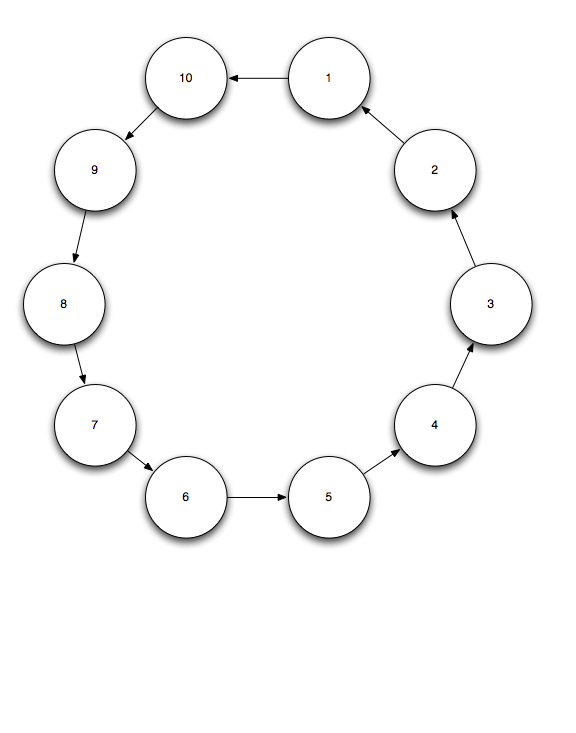
\includegraphics[width=\linewidth]{figures/heartbeat-protocol-arrangement}
\end{figure}

We deployed 10 nodes in a room in our test lab, which results in a fully
connected network. Therefore only one heartbeat chain loop is formed.

The heartbeat procotol arrangement is simple. Every node is sending heartbeat to
previous node except the first node, which sends to the last. For example, node
1 receives heartbeat message from node 2, node 2 receives heartbeat message from
node 3, etc. Figure~\ref{fig:heartbeat-protocol-arrangement} illustrates the
arrangement for this experiment.

\section{Hardware Platform}

\begin{figure}[h!]
\caption{An WuDevice}
\label{fig:wudevice}
\centering
    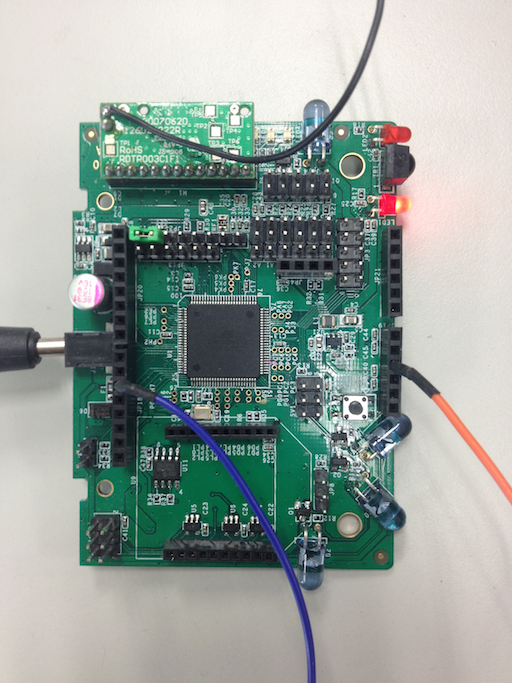
\includegraphics[width=\linewidth]{figures/wudevice}
\end{figure}

All boards are equipped with an Atmel ATmega1280-16AU 8-bit microcontroller with
4K of EEPROM and 64k of flash. The boards hardware design is based upon Arduino
hardware referenced design, in addition, every board has wires for mounting
multiple wireless protocol adapters such as ZWave, ZigBee. In the following
experiments, every board is only equipped with a ZWave adapter, and only
communicating through ZWave.  Every board is also pre-installed with a modified
version of NanoVM~\cite{Harbaum2006} called “NanoKong”~\cite{Su} that supports all the basic
WuKong framework protocols including the new additions from the work in the
previous chapter.  A PC with wireless access is dedicated for hosting the WuKong
Master software which is responsible for managing WuKong applications for the
whole system and serves as a mean to present an interface to the users.  Three
boards will be used in the experiments below. One of them is equipped with
a light sensor that returns a byte indicating the light level around the sensor.
The rest are equipped with a relay which each controls the power supply of
a lamp.  An additional board with the same hardware specification is used as
a gateway between the Master and the sensor network.

\section{Experimental Setup}

\begin{table}
\centering
\caption{Node setup}
\label{tbl:setup}
  \begin{tabular}{|l|l|}
  \hline
  \textbf{Node Id} & \textbf{Equipped resources} \\
  \hline
  1(2) & Light Actuator \\
  \hline
  2(4) & Numeric Controller, Threshold, Light Sensor \\
  \hline
  3(5) & Light Actuator \\
  \hline
  4(6) & Light Actuator \\
  \hline
  5(7) & Light Actuator, Light Sensor \\
  \hline
  6(10) & Light Actuator \\
  \hline
  7(12) & Light Actuator \\
  \hline
  8(13) & Light Actuator \\
  \hline
  9(14) & Light Actuator \\
  \hline
  10(15) & Light Actuator \\
  \hline
  \end{tabular}
\end{table}

Ten WuDevices are installed throughout our testbed. Every WuDevice will be
able to talk to each other directly forming a fully connected network. Eight of them are
equipped with light actuators. Two of them have light sensors. Only one of them
has user input device (Numeric Controller), and Threshold. We simulate a node
failure by removing power supply of a WuDevice. Every device communicates
wirelessly through ZWave adapter. The setup is shown in table~\ref{tbl:setup}

\section{Mapping results}

\begin{table}
\centering
\caption{Strips}
\label{tbl:mapping-result}
  \begin{tabular}{|l|l|}
  \hline
  \textbf{Application Component} & \textbf{Mapped nodes (strip)} \\
  \hline
  Numeric Controller & 2 \\
  \hline
  Light Sensor & 2, 5 \\
  \hline
  Light Actuator & 1, 3, 4, 5, 6, 7, 8, 9, 10 \\
  \hline
  Threshold & 2 \\
  \hline
  \end{tabular}
\end{table}

The result of the mapping and the strips are shown in
table~\ref{tbl:mapping-result}. Each row represents each component in the
application, where strips are ordered from the left.


%\section{Mapping method}

%Deployments with different strip ordering method, such as first-fit, last-fit,
%closest-fit, will be performed to compare their effects on system performance.

%As first-fit was introduced in eariler chapter at chapter~\ref{c:design}, the
%other methods that will be used in the experiment are introduced here.

%Last fit is exactly first fit but reversing the order at the end.
%Closest fit sorts the strips by the order of the histogram of number of unique
%capability a node has.


\section{Results}
\label{s:results}

\begin{figure}[h!]
\caption{Average recovery time and message overhead over 5 deployments for each
node failure as the first failure}
\centering
    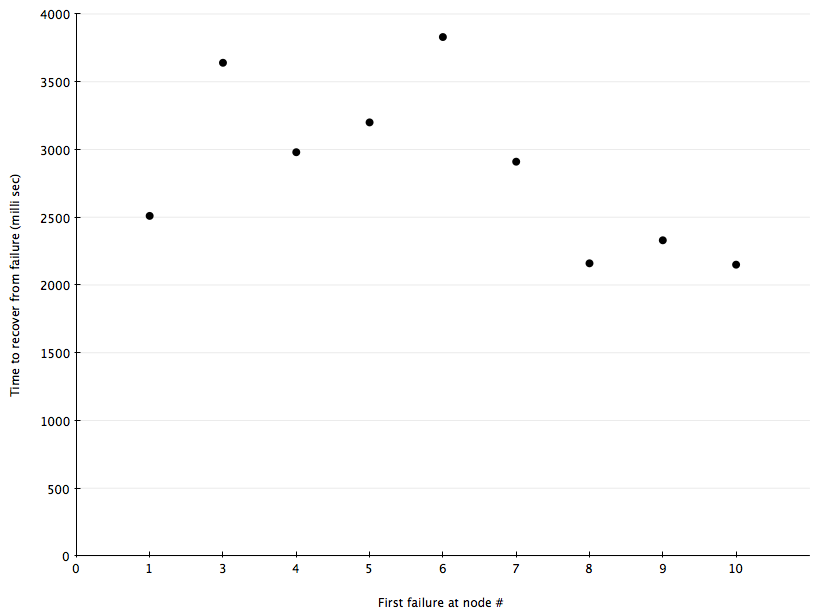
\includegraphics[width=\linewidth]{figures/results-average-recovery-time-plus-message-overhead}
\label{fig:results-average-recovery-time-plus-message-overhead}
\end{figure}

\begin{table}
\centering
\caption{Strip memory overhead in bytes}
\label{tbl:results-memory-overhead-strip}
  \begin{tabular}{|l|l|}
  \hline
  \textbf{Application Component Strip} & \textbf{Memory size (bytes)} \\
  \hline
  Numeric Controller & 2 \\
  \hline
  Light Sensor & 2 \\
  \hline
  Light Actuator & 18 \\
  \hline
  Threshold & 2 \\
  \hline
  \end{tabular}
\end{table}

The results for memory overhead by strips before failures are consistent, as
each node address takes only one byte, the other byte is used in our unique
identification system to recognize wuobject on a node. All failovers in
deployments have been swift and correct.

The figure~\ref{fig:results-average-recovery-time-plus-message-overhead}
illustrates the average recovery time and message overhead over 5 deployments
for each node failure in Strip for Light Actuator as first failure in the
system. The first failure should on average takes the longest time and higher
message overhead compared to consequent failures. Therefore measuing the
performance for each node failure as first failure would give us how the system
would perform the worst overall. The results carried over even in different
strip orders for Light Actuator Strip since the ordering is just a matter of
permuting the results as shown in the results.

The recovery time for most nodes were averaging around 2500 milli-seconds, node
3 and node 6 are found out that their radios were a little defective (without
antenna) after the experiments therefore it took longer to complete the
recovery. It is clear that the results have shown were pretty consistent as
there were only a constant number of nodes that needed to contact to recovery
regardless of how many strips the node contained. The time it took is reasonable
given the small network.

% Complexity analysis
% TODO:Just pasted, need revision
The lower bound of message overhead for heartbeats arranged in a daisy chain
loop in a network of size n is $\Omega(n)$, the upper bound is also $O(n)$, since
there is only one message sent by a node at any given moment.

% Complexity analysis
% TODO:Just pasted, need revision
For an application with m components deployed to a network with n nodes where
n > 1, the lower bound of memory overhead of the strips for a random member in
the network is $\Omega(1)$ since a node must carry at least one strip and lowest
member requirement of a strip is 2. The upper bound is $O(m*n)$ since the strips
could span the whole network. But in reality, since the nodes typically have
fixed memory and fixed capability for the duration of the lifetime in the
network, the upper bounds cannot grow indefinitely. The memory overhead a strip
could impose on a node is determined by node's capability and memory size.


% Complexity analysis
% TODO:Just pasted, need revision
The lower bound of message overhead by the reconfiguration protocol
with one node failure in the same network is $\Omega(1)$, since if there is only
one component with 2 members on the failed node, the detector would only need to
send 1 messages to the remaining strip member of the failing node, and none if
the component is not connected to any other components, and finally 1 more
message to get the information from the nodes monitored by the failed node. The
upper bound is $O(n + m)$ since if the failed node carried m components where each
strip contains n members, the detector would have to send (n-2) messages to all
functioning members of the m strips carried excluding itself plus the messages
to all other strip heads connected to the failing node. 

The time to recover highly depends on the messages sent for the reconfiguration
and the detection time. The lower bound is $\Omega(1)$ with the same assumption
with constant component and members, but the upper bound is $O(b + n + m)$ where
b is the heartbeat period.

The cost for time for recover is the time itself. Time is the overhead. Thus the
longer time it take to recover the higher the overhead. By setting a shorter
heartbeat period, it would take a shorter time to recover, thus a lower
overhead. I assume every message takes at least a fixed amount of time, and
there need at least amount of messages to recover, so the more messages it takes
to recover, the longer the time it will take to recover. Here it is assumed that
heartbeat messages are never lost/dropped, and in-node computation take
negligible amount of time thus it is ignore. If it is about the message overhead
within a certain time period, then of course the higher the period the lower the
message overhead.

% TODO:Just pasted, need revision
A small network with around 10 nodes with a 5-component application can operate
if each node could dedicate at most 50 bytes of memory to strips (assuming one
byte node addressing), and equipped with radios and battery capable of handling
extra 15 messages for reconfiguration messages per failure. The requirements are
reasonable since most embedded devices have at least 4K of EEPROM to store
strips, and have radios with throughputs of 40kbps, thus the ideal recovery time
without in-node processing and interference and retry would be around
3 milli-seconds.

Depending on the wireless protocol used, a ZWave network can include up to 232
nodes, which is pretty big for most real world deployments. Strips can still be
run in network of size like this, since a 4K EEPROM could hold up to 400 members
per strip for a 5 component application.

% Probably move it to future work? Probably don't do it.
%Of course there are a lot of room for improvements. For example, if we want to
%go beyond this limitation of 232 nodes by Zwave, one of the ways we could do is
%to build another zwave network and have a routing agent to route messages
%between networks. And we would also want to handle network partitions. One of
%the possible research directions is to merge the partitions back to one if they
%come back together, or by using some arbitrary flags to indicate primary
%components in the network to eliminate redundant commanding network components.
%Nonetheless, it is also an opportunity to look into multi-hop networks since
%heartbeats protocols are designed with single-hop network in mind, whether we
%could change the protocol to handle multi-hop is also a big challenge a future
%research could take on.
